\documentclass{article}
\usepackage{iclr2026_conference}
\usepackage{amsmath,amssymb}
\usepackage{booktabs}
\usepackage{graphicx}
\usepackage{microtype}
\usepackage{url}
\usepackage[table]{xcolor}
\usepackage[colorlinks=true,linkcolor=black,citecolor=black,urlcolor=blue]{hyperref}
% Set the PDF metadata explicitly: hyperref cannot derive it from a title and
% author block that contain \ and \And.
\hypersetup{
  pdftitle={Competition Produces the Experts: Routing LoRA Specialists in a Learned Safety Trait Space},
  pdfauthor={Mark Lovett, Denis Lim, Soroush Vosoughi},
  pdfsubject={Manuscript, incomplete draft},
}
\graphicspath{{figures/}}

\title{Competition Produces the Experts: Routing LoRA\\Specialists in a Learned Safety Trait Space}

\author{
  Mark Lovett\thanks{Correspondence: \texttt{mark.lovett.gr@dartmouth.edu}} \\
  Dartmouth College \\
  \And
  Denis Lim \\
  Cambridge AI Safety Hub \\
  \And
  Soroush Vosoughi \\
  Dartmouth College
}

\begin{document}
\maketitle

\begin{abstract}
Mixture-of-experts systems assume the experts already exist. Someone partitions the data, trains one
adapter per shard, and the router learns to pick among them. We remove that step. Seven LoRA adapter
pairs are placed in a learned seven-axis safety trait space and left to compete for prompts under a
proportional allocation rule, so the partition is an outcome of training rather than an input to it.
A single parameter, the competitive reach $\sigma$, controls how localised each pair's claim is, and
the router is the same allocation rule evaluated at the positions the pairs converged to.
On a held-out pool of 5{,}671 prompts the routed ensemble reaches 1.9459 mean NLL against 2.0151 for
a generalist trained on exactly the same prompts, a 3.4\% reduction, with an oracle floor of 1.8857.
Combining the experts' sequence likelihoods rather than committing to one widens the margin to 0.110,
a 5.4\% reduction. Three design choices matter and one does not. Training every pair on every prompt
in proportion to its share beats a top-3 gate by 0.028 NLL, weighting the loss by share beats unit
weighting by 0.010, and collapsing to a single hard-routed winner is the only configuration that
loses to the generalist as a selector --- though it wins as a mixture, so that conclusion is
metric-dependent. Unit weighting halves router agreement with the oracle, from 0.705 to 0.540,
because it discards the signal the router routes on. Sweeping $\sigma$ over a fourteen-fold range
moves the oracle by only 0.022 NLL but the router by 0.055: $\sigma$ governs how much of the
available specialisation the router can reach, not how much exists. Where the pairs \emph{start}
decides the outcome only when capacity is scarce: initialising at an equilibrium of the game solved
against the empirical prompt measure is worth 0.013 to 0.036 NLL at four pairs or fewer, enough to
turn routing from a loss into a gain at two pairs, and nothing at five or more. The gain persists
from 1.2B to 7B parameters and across three model families, and the learned positions are identical
across model scales.
\end{abstract}

\section*{Status of this draft}
\textbf{This manuscript is an incomplete draft.} Four things are open. The replication in
Section~\ref{sec:limits} covers four data splits; further splits are running and the error bars will
tighten. The reach sweep at the game equilibrium (Section~\ref{sec:init}) is complete on one split
and in progress on a second, so its smoothness result is reported as measured but not yet replicated,
and the control that would establish its cause has not been run. The Gemma-3-1B generalist had not
converged at the round budget, so its apparent gain is inflated and is excluded from the scaling
trend. The companion paper that supplies the game-theoretic result is unpublished, and
\citet{lovett2026influencer} is a placeholder citation.

\section{Introduction}
A mixture-of-experts model routes each input to a subset of specialised parameters
\citep{shazeer2017moe,fedus2022switch}. The recent parameter-efficient version of this idea reuses
LoRA adapters as the experts \citep{hu2022lora,huang2024lorahub,yadav2024moerging}. In nearly all of
this work the experts come first. A practitioner splits the training data by task, domain or
language, fine-tunes one adapter per shard, and then fits a router over the resulting library. The
partition is a design decision, and a router can only be as good as the partition it inherits.

We start one step earlier and let the experts find their own data. Adapters are given positions in a
learned trait space and compete for training prompts. At each point of the space an adapter's claim
is a Gaussian kernel centred on its position, and each adapter receives a share of that point
proportional to its claim relative to the others. Adapters then move toward the prompts they are
winning, and the partition falls out of the competition instead of being imposed on it.

The model behind this is the influencer's game of \citet{lovett2026influencer}, which we describe in
Section~\ref{sec:game}. It is a general account of $N$ players choosing positions in a space and
splitting a resource by proportional allocation, and it answers exactly the question an ensemble
designer needs answered: when do competitors converge on the same position and when do they separate
into niches? The answer turns on one quantity, the competitive reach $\sigma$ measured against the
spread of the resource. Above a threshold $\sigma_0^*$ every player sits at the resource-weighted
mean and nobody specialises, which is the classical minimum-differentiation result. Below it the
symmetric equilibrium is unstable and the players fragment. We run the whole study below
$\sigma_0^*$ and use $\sigma$ as the dial that sets how finely the partition is drawn. That single
scalar replaces the entire design decision of how to shard the data.

The result is a mixture of experts in which no partition was ever specified, and we make five claims
about it. First, a competitively positioned ensemble of seven LoRA pairs beats a generalist trained
on exactly the same prompts, by 0.069 mean NLL on a held-out pool of 5{,}671 safety prompts
(Section~\ref{sec:routing}); the comparison is prompt-matched round by round, so the generalist sees
the same data in the same order. Combining the experts rather than selecting one widens that to 0.110
(Section~\ref{sec:mixture}). Second, the standard sparse-MoE recipe is the wrong one here: dense
proportional training beats a top-3 gate, share-weighted loss beats unit weighting, and hard
single-expert routing is the only setting that loses to the generalist --- as a selector. Under the
mixture the same arm wins, so that particular conclusion depends on which number one reports, and we
report both. Unit weighting does the most damage, cutting router agreement with the oracle from
0.705 to 0.540.

Third, sweeping $\sigma$ across ten values separates two effects that are easy to conflate
(Section~\ref{sec:sigma}). The specialists are about equally good at every $\sigma$, with an oracle
spread of 0.022 NLL over a fourteen-fold range of reach, while the router moves two and a half times
as much. Reach controls how much specialisation the router can use, not how much exists, and the arm
closest to $\sigma_0^*$ gives up more than half of it. Fourth, where the pairs begin matters, but only
when capacity is scarce (Section~\ref{sec:init}). Starting them at an equilibrium of the game solved
against the empirical prompt measure, rather than at the uninformative start the earlier arms used,
is worth 0.013 to 0.036 NLL at four pairs or fewer and nothing at five or more; at two pairs it is
the difference between routing hurting and helping. It also moves the capacity threshold down by one
pair, so part of what looked like a property of the method was a property of its initialisation.
Fifth, the effect is not an artefact of one base model (Section~\ref{sec:scale}): the gain holds at
1.5B, 3B and 7B parameters and on a second model family, decaying slowly with scale. Because
positions are learned in the trait space rather than in the model, they come out identical across
scales.

\section{Related work}
\textbf{Sparse mixtures of experts.} Conditional computation routes each token or example to a few of
many expert subnetworks \citep{shazeer2017moe}. Switch Transformer simplifies the gate to a single
expert per token and exposes the load-balancing problem that dominates practical MoE training
\citep{fedus2022switch}; expert-choice routing inverts the assignment so experts select tokens
instead \citep{zhou2022expertchoice}. These systems learn the router jointly with experts that have
no prior identity, and the resulting specialisation is famously hard to interpret. Our experts have
positions in a space with named axes, and the router is a closed-form function of those positions
rather than a separately trained network.

\textbf{Adapter libraries and post-hoc routing.} A second line of work treats independently trained
LoRA adapters as a library to be composed. LoraHub learns mixing coefficients over a set of
task-specific adapters for an unseen task \citep{huang2024lorahub}; related work merges adapters
arithmetically \citep{ilharco2023task} or attaches a learned gate over frozen experts. The survey of
\citet{yadav2024moerging} calls this family model MoErging and observes that essentially all of it
takes the expert set as given. That assumption is what we relax: our adapters are trained
simultaneously, and each one's training distribution is determined by what it wins from the others.

\textbf{Spatial competition.} Positioning competitors so as to capture demand is a long literature
beginning with \citet{hotelling1929stability} and extended by \citet{salop1979monopolistic} and
\citet{downs1957economic}. Its classical result is minimum differentiation, competitors converging on
the same position, which \citet{eaton1975principle} showed depends on the number of players and the
shape of demand. \citet{lovett2026influencer} generalise these models to $N$ players in $L$
dimensions with an arbitrary influence kernel and resource distribution, and derive the threshold
that separates convergence from niche formation. Section~\ref{sec:game} states the parts we use.

\textbf{Safety evaluation.} The trait space is built from seven public safety benchmarks covering
harmful response \citep{ji2023beavertails}, hallucination \citep{li2023halueval}, jailbreak
robustness \citep{chao2024jailbreakbench}, privacy leakage \citep{ai4privacy2023}, over-refusal
\citep{cui2024orbench}, prompt injection, and policy violation \citep{wang2023donotanswer}. We use
them to define directions in embedding space rather than as a leaderboard.

\section{The influencer's game}
\label{sec:game}
The ensemble is built on the influencer's game of \citet{lovett2026influencer}, so we state the model
and the one result we rely on. There are $N$ players. Player $i$ chooses a position $x_i$ in a
compact strategy space $\mathbb{D} \subseteq \mathbb{R}^L$, and exerts an influence $f_i(x_i, b) > 0$
at each point $b$ of a resource space $\mathbb{B}$. A resource distribution $B(b)$ says how much is
available at each point. Player $i$'s share at $b$ is its influence relative to the field, and its
payoff is that share integrated against the resource,
\begin{equation}
G_i(\mathbf{x}, b) = \frac{f_i(x_i, b)}{\sum_j f_j(x_j, b)}, \qquad
u_i(\mathbf{x}) = \int_{\mathbb{B}} B(b)\, G_i(\mathbf{x}, b)\, \mathrm{d}b .
\label{eq:game}
\end{equation}
The shares sum to one at every point, so the game is constant-sum: what one player gains another
loses. Players do not choose which resource to pursue, only where to stand, and everything about who
serves what follows from the geometry. Hotelling's location model, Salop's circular market and the
spatial models of voting are all special cases \citep{hotelling1929stability,salop1979monopolistic,downs1957economic}.

With a log-concave kernel the game has a unique symmetric Nash equilibrium, and for the Gaussian
kernel it sits at the resource-weighted mean $x^* = \mathbb{E}_B[b]$: every player stands in the
middle and takes an equal $1/N$ share. Whether players stay there is a separate question, and it is
the one that matters for building an ensemble. \citet{lovett2026influencer} show that for a Gaussian
kernel of standard deviation $\sigma$ the symmetric equilibrium is locally stable exactly when
\begin{equation}
\sigma > \sigma_0^* := \sqrt{\frac{N-2}{N-1}}\;\sigma_B,
\label{eq:threshold}
\end{equation}
where $\sigma_B$ is the spread of the resource distribution. The condition compares how far a
player's influence reaches against how spread out the resource is. When reach is broad relative to
the resource, a player who steps away from the centre loses share everywhere and the incentive is to
crowd in. When reach is narrow, stepping toward a local peak of $B$ wins that peak outright and
costs little elsewhere. Below $\sigma_0^*$ the symmetric equilibrium destabilises and gives way to a
cascade of bifurcations: first a dispersed configuration, then limit cycles, then asymmetric
clusters, with players settling around the modes of the resource landscape.

This is a description of how specialisation arises without anyone designing it, which is why we use
it. Three properties carry over directly. The competition is constant-sum, so an adapter can only
gain training signal by taking it from another, and no coordination mechanism or load-balancing loss
is needed to stop them all learning the same thing. The partition is an equilibrium rather than an
input, so the number of niches and their boundaries are determined by the resource landscape.
And a single scalar $\sigma$, read against a threshold that the theory gives in closed form, controls
how finely the space is divided.

Mapping the game onto the ensemble is direct. The players are LoRA adapters. The strategy space is a
learned trait space over prompts. The resource distribution is the density of training prompts in
that space, so $B$ is estimated from data rather than assumed. A player's share $G_i$ becomes the
weight that prompt carries in that adapter's loss, so winning share and getting training signal are
the same thing. The only quantity we set by hand is $\sigma$, and we set it as a fraction of the
$\sigma_0^*$ that Equation~\ref{eq:threshold} produces for our landscape.

The correspondence is not exact. The theory describes fixed points of a positioning game with a
static resource and stateless players, while our adapters accumulate weights and change what they are
good at as they train. We therefore use the theory to choose and interpret $\sigma$, not to predict
where any particular adapter ends up.

\section{Method}
\label{sec:method}
\subsection{Trait space}
Prompts are embedded with Qwen3-Embedding-8B, quantised to AWQ-INT4, using last-token pooling at a
512-token limit and $L_2$ normalisation \citep{qwen2025embedding}. Each of the seven axes is a
direction in that 4096-dimensional space, learned from one benchmark. For axis $j$ we take the
benchmark's positive and negative examples, compute a shrinkage-regularised Fisher discriminant
\citep{fisher1936lda}
\begin{equation}
w_j = \big(0.9\,S_w + 0.1\,\tfrac{\operatorname{tr}S_w}{D} I\big)^{-1}(\mu_+ - \mu_-),
\end{equation}
orthogonalise it against the axes already accepted, and calibrate it by the 5th percentile of the
negative projections and the 95th of the positive. Five of the seven axes then replace this
label-separating direction entirely with a one-versus-rest direction that separates the benchmark
from the other six; harm and hallucination blend the two at weight $0.35$. Axis scores are
residualised against earlier axes and passed through a per-axis empirical CDF, so the trait space is
the unit cube $[0,1]^7$ and each axis is marginally uniform on the corpus. Harm and hallucination are
scored on response embeddings, the other five on prompt embeddings.

The resource distribution $B(b)$ is a Gaussian kernel density estimate of all 28{,}355 corpus prompt
coordinates, evaluated on a $3^7 = 2187$-point grid at bandwidth $0.08$. Grid spacing is $0.5$ and
the bandwidth is $0.08$, so $B$ is close to a nearest-cell histogram; it is a coarse summary of where
prompts live, not a smooth density.

\subsection{Playing the game over adapters}
We instantiate Equation~\ref{eq:game} with $N = 14$ adapters, indexed $i$, holding positions
$x_i \in [0,1]^7$ and grouped into seven co-located pairs. The influence kernel is Gaussian with
$\Sigma = \sigma^2 I_7$, so $\sigma$ in our configs is a standard deviation in trait-space units,
\begin{equation}
f_i(x_i, b) = \exp\!\big(-\tfrac12 (x_i - b)^\top \Sigma^{-1}(x_i - b)\big),
\label{eq:share}
\end{equation}
and a pair's share is the sum of its two members' shares. Positions are initialised by gradient
ascent on $u_i$ over the KDE grid, paired by nearest neighbour, and re-solved from the paired state.
Positions then move once per round. Adapter $i$ is pulled toward the centroid of the round's prompts
$\{b_m\}$ weighted by $G_i(1-G_i)$, and takes a fraction $\beta$ of the way there,
\begin{equation}
x_i \leftarrow (1-\beta)\,x_i + \beta\,\frac{\sum_m G_i(b_m)\,(1 - G_i(b_m))\,b_m}
                                            {\sum_m G_i(b_m)\,(1 - G_i(b_m))}, \qquad \beta = 0.5 .
\label{eq:posupdate}
\end{equation}
The weight is not arbitrary. Under isotropic $\Sigma$ the payoff gradient of Equation~\ref{eq:game}
is $\nabla_{x_i} u_i = -\sum_k B(b_k)\,G_i(1-G_i)\,\Sigma^{-1}(x_i - b_k)$, so the same $G_i(1-G_i)$
that appears in the gradient appears in the update, and a step toward this centroid points along the
gradient. The adapters are climbing the payoff the theory analyses rather than following a
convenience heuristic, which is what lets us read the sweep against $\sigma_0^*$.

The factor has a plain reading. $G_i(1-G_i)$ is largest where adapter $i$ holds about half the share
and near zero where it holds almost all or almost none. A prompt already won outright exerts no pull,
because there is nothing more to gain there; a prompt that is genuinely contested pulls hardest. Two
details follow from the code and are worth stating. The mass is computed over the whole round batch,
not just the prompts an adapter trains on, so a top-$k$ gate changes what an adapter learns but not
where it moves. And it is deliberately not renormalised per prompt, since dividing through would tilt
the step off the gradient direction. Co-located partners see identical $G_i$ and therefore take
identical steps, so a pair staying together is a prediction of the update rule that we audit, not a
constraint we impose.

For the multivariate case the threshold of Equation~\ref{eq:threshold} uses
$\sigma_B = \sqrt{\Lambda_{\max}(\Sigma_B)}$, the largest standard deviation of the resource
distribution, since instability appears first along the most varied direction. On our landscape, with
$N = 14$, this gives $\sigma_0^* = 0.40977$. All ten arms use $\sigma < \sigma_0^*$, so the whole
study sits below the threshold, in the regime where the symmetric equilibrium is unstable and the
pairs separate. We never run the stable regime, where the theory predicts every adapter would collapse
onto the resource-weighted mean and the ensemble would reduce to a generalist.

\subsection{Training and routing}
Each round draws a disjoint batch of 1{,}654 training prompts; twelve rounds cover the 19{,}848
training prompts exactly once. Within a round, pair $p$ trains on the prompts it is allocated, with
per-example loss weight equal to its share. LoRA uses rank 16, $\alpha=32$, dropout $0.05$ on all
attention and MLP projections, learning rate $2\times10^{-4}$, effective batch 16, one epoch per
round, and adapters accumulate across rounds.

Three choices in this loop are free, and Section~\ref{sec:routing} varies them one at a time. The
first is $k$: how many of the seven pairs are given a prompt at all. At $k=7$ every pair trains on
every prompt. At $k=3$ only the three largest shares survive and are renormalised, so four pairs never
see that prompt. The second is how those $k$ are picked. \emph{Argmax} takes the $k$ largest shares
deterministically. \emph{Sampled} draws $k$ pairs without replacement with probability proportional
to share, so a pair with a small share still occasionally trains on a prompt it did not win. The third
is what a selected pair does with the prompt. Under \emph{share} weighting the per-example loss is
multiplied by $G_p$, so a pair that barely won a prompt takes a correspondingly small gradient step
on it. Under \emph{unit} weighting every selected pair treats the prompt identically, which discards
the share magnitude and keeps only the selection. Hard $k{=}1$ is the corner of this design where a
single sampled winner takes the prompt at unit weight, giving each pair a disjoint seventh of the
data; it is the compute-matched control and the closest setting to standard top-1 MoE.

At evaluation the router is Equation~\ref{eq:share} evaluated at the final-round positions, with the
same $\sigma$ used in training. There is no separately trained gate: routing at test time is the same
allocation rule that distributed the training data, read off the positions the competition produced. We report three quantities on
the held-out pool, all as means over examples of the per-example token-mean NLL:
\emph{oracle}, the per-prompt minimum over the seven pair adapters;
\emph{router}, the share-weighted expectation $\sum_p G_p(b_m)\,\mathrm{NLL}_p(m)$;
and \emph{pooled}, a single generalist adapter. Router/oracle agreement is the fraction of prompts on
which the highest-share pair is also the lowest-NLL pair. Agreement uses the argmax rule while the
router NLL uses the expectation, so the two are not two views of one decision.

The generalist is trained by replaying the same twelve round batches, de-duplicated so it sees each
round's 1{,}654 prompts once, with identical LoRA hyperparameters. Every arm draws from the same
manifest, so all rounds are set-identical across arms and one generalist is matched to all of them.
Matching is on data, not compute: with dense allocation each of the seven pairs trains on every
prompt, so the ensemble consumes roughly seven times the gradient steps.

\section{Experimental setup}
The corpus is 28{,}355 prompts drawn from seven benchmarks, split 70/10/20 into 19{,}848 train,
2{,}836 validation and 5{,}671 test. The test pool is capped at 1{,}000 records per benchmark;
JailbreakBench (40) and OR-Bench (631) fall below the cap. Unless stated otherwise the base model is
Qwen2.5-1.5B-Instruct \citep{qwen2024qwen25}, results are at round 11, and $\sigma/\sigma_0^* = 0.50$.
Runs used a single A100-80GB; one arm takes about 2.6 GPU-hours.

\section{Routing design}
\label{sec:routing}
Table~\ref{tab:routing} and Figure~\ref{fig:routing} cross the three factors defined at the end of
Section~\ref{sec:method}: how many pairs train on a prompt, whether those pairs are chosen by argmax
or sampled, and whether the loss is weighted by share or uniformly. Every arm shares one generalist
and one set of test prompts, so the columns are directly comparable.

\begin{table}[t]
\centering
\caption{Routing design at $\sigma/\sigma_0^* = 0.50$, round 11, $n=5{,}671$. All five arms share one
data-matched generalist, so \emph{pooled} is identical at 2.0152. \emph{Expected} commits to one
expert per prompt in proportion to share; \emph{mixture} combines the experts' sequence likelihoods
(Section~\ref{sec:mixture}); \emph{uniform} is the same mixture with the router's weights replaced by
$1/K$, and isolates what the learned weights contribute. All three are margins over pooled, and more
negative is better.}
\label{tab:routing}
\small
\setlength{\tabcolsep}{3.8pt}
\begin{tabular}{llccccccc}
\toprule
Arm & Selection & $k$ & Loss & Oracle & Expected & Mixture & Uniform & Agree. \\
\midrule
Soft $k{=}7$      & argmax, all    & 7 & share & 1.8857 & $-0.0693$ & $\mathbf{-0.1095}$ & $-0.0661$ & 0.705 \\
Soft $k{=}3$      & argmax top-3   & 3 & share & 1.9112 & $-0.0413$ & $-0.0834$ & $-0.0401$ & 0.700 \\
Soft $k{=}3$ unit & argmax top-3   & 3 & unit  & 1.9379 & $-0.0313$ & $-0.0505$ & $-0.0225$ & 0.540 \\
Sampled $k{=}3$   & sampled        & 3 & unit  & 1.9437 & $-0.0282$ & $-0.0450$ & $-0.0167$ & 0.545 \\
Hard $k{=}1$      & sampled winner & 1 & unit  & 1.9601 & $+0.0156$ & $-0.0341$ & $+0.0090$ & 0.706 \\
\bottomrule
\end{tabular}
\end{table}

\begin{figure}[t]
\centering
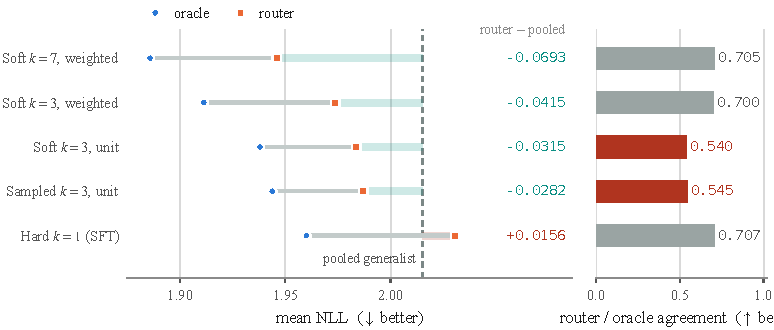
\includegraphics[width=\textwidth]{fig_routing_ablation.pdf}
\caption{Five routing designs against the shared generalist (dashed). The bar between router and
generalist is the margin; only hard $k{=}1$ falls on the wrong side of it. Unit weighting (rows 3 and
4) halves agreement with the oracle without moving the NLL much.}
\label{fig:routing}
\end{figure}

Dense allocation wins. Training all seven pairs on every prompt in proportion to share beats a top-3
gate by 0.028 NLL, and the gap is visible in the oracle as well as the router, so it is the
specialists that are better, not just the routing. This runs against the usual sparse-MoE
justification, but the economics differ: our experts are rank-16 adapters on a shared base, so
activating all seven costs seven adapter forward passes rather than seven copies of the model.

Share weighting matters more than the gate does. Holding $k=3$ and changing only the loss weight
costs 0.010 NLL and drops agreement from 0.704 to 0.540. Unit weighting trains every selected pair
equally hard on a prompt regardless of how strongly it claimed that prompt, which flattens exactly
the signal the router later uses. The two unit-weighted arms are also the only ones whose inter-axis
NLL falls below 2.05, meaning the pairs have become more alike.

Hard routing loses \emph{as a selector}: sampling a single winner per prompt gives each pair one
seventh of the data and produces an ensemble worse than the generalist by 0.016 expected NLL. Its
agreement stays high at 0.706 because the pairs remain distinct, but there is not enough training
signal in each. That arm is the compute-matched control and the setting closest to standard top-1
MoE. We previously reported this as the one configuration that loses to the generalist, and that
statement is metric-dependent: under the sequence-level mixture the same arm \emph{wins}, at
$-0.0341$. What hard routing damages is each expert's competence, not the ensemble's ability to
combine them, and a combination rule that can hedge across experts recovers most of the loss. The
ordering of the five designs is otherwise identical under both metrics, so no other conclusion in
this section turns on the choice.

The uniform column separates the router's contribution from the ensemble's. Replacing the learned
weights with $1/K$ costs 0.043 NLL on the dense arm ($-0.1095 \to -0.0661$), so roughly 40\% of the
mixture margin is attributable to \emph{where} the router places its mass rather than to averaging
alone. On the hard arm the same substitution flips the sign back to $+0.0090$: with one-seventh-trained
experts, uniform averaging is worse than the generalist and only the learned weights rescue it.

\section{Trait space}
\label{sec:trait}
Figure~\ref{fig:traitspace} shows where prompts sit and where the pairs settle. Because each axis is
mapped through its own empirical CDF, the marginals are uniform by construction and all structure is
in the joint distribution. The seven pairs do not spread evenly: two share a dominant harm
coordinate, and the privacy axis is not claimed as any pair's argmax. The pair-to-axis map is
therefore not a bijection, which is worth stating plainly, since it would be easy to assume seven
pairs and seven axes align one-to-one. They do not, and the routing gain does not require them to.

\begin{figure}[t]
\centering
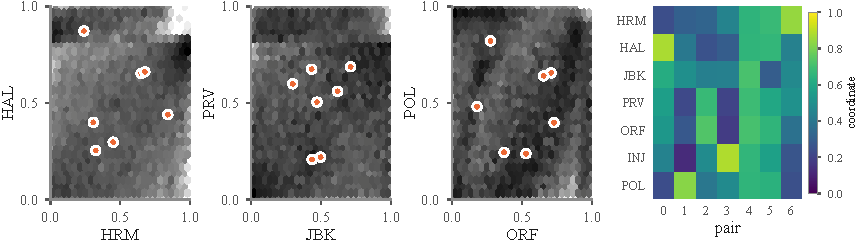
\includegraphics[width=\textwidth]{fig_trait_space.pdf}
\caption{Left three panels: density of the 28{,}355 corpus prompts on three axis pairs (darker is
denser), with the seven final pair positions in orange. Right: the same positions as coordinates,
one column per pair. Axes are HRM harm, HAL hallucination, JBK jailbreak, PRV privacy, ORF
over-refusal, INJ injection, POL policy.}
\label{fig:traitspace}
\end{figure}

\section{Competitive reach}
\label{sec:sigma}
We sweep $\sigma/\sigma_0^*$ from 0.70 down to 0.05, a fourteen-fold range in reach, changing nothing
else. Table~\ref{tab:sigma} and Figure~\ref{fig:sigmanll} give the result.

\begin{table}[t]
\centering
\caption{Competitive reach sweep, Qwen2.5-1.5B, round 11, $n=5{,}671$. Pooled is 2.0151 for every
row. Own and other are the mean NLL on the axis a pair owns and on the remaining six.}
\label{tab:sigma}
\small
\begin{tabular}{ccccccc}
\toprule
$\sigma/\sigma_0^*$ & $\sigma$ & Oracle & Router & Router$-$pooled & Agree. & Own / other \\
\midrule
0.70 & 0.2868 & 1.8912 & 1.9781 & $-0.0370$ & 0.627 & 1.799 / 2.007 \\
0.60 & 0.2459 & 1.8833 & 1.9528 & $-0.0623$ & 0.701 & 1.792 / 2.119 \\
0.55 & 0.2254 & 1.8877 & 1.9498 & $-0.0653$ & 0.703 & 1.811 / 2.158 \\
0.50 & 0.2049 & 1.8857 & 1.9459 & $-0.0692$ & 0.705 & 1.804 / 2.228 \\
0.45 & 0.1844 & 1.8993 & 1.9539 & $-0.0612$ & 0.645 & 1.815 / 2.232 \\
0.40 & 0.1639 & 1.8963 & 1.9470 & $-0.0681$ & 0.700 & 1.810 / 2.284 \\
0.30 & 0.1229 & 1.8883 & 1.9445 & $-0.0706$ & 0.710 & 1.799 / 2.328 \\
0.20 & 0.0820 & 1.8830 & 1.9234 & $-0.0916$ & 0.795 & 1.793 / 2.390 \\
0.10 & 0.0410 & 1.8959 & 1.9452 & $-0.0699$ & 0.688 & 1.823 / 2.334 \\
0.05 & 0.0205 & 1.9050 & 1.9464 & $-0.0686$ & 0.785 & 1.794 / 2.373 \\
\bottomrule
\end{tabular}
\end{table}

\begin{figure}[t]
\centering
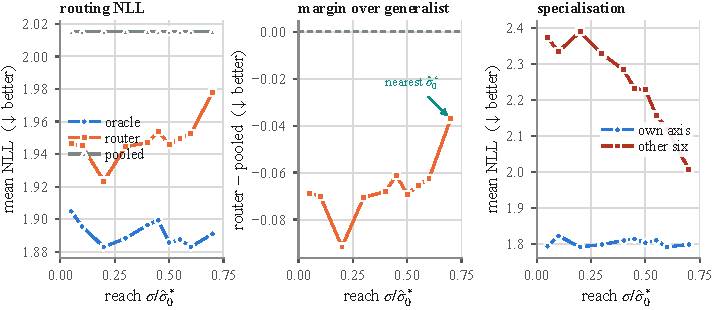
\includegraphics[width=\textwidth]{fig_sigma_nll.pdf}
\caption{Left: the three NLLs against competitive reach. Right: the router's margin over the
generalist. The oracle is nearly flat while the router is not, so reach controls how much
specialisation the router can use rather than how much the specialists have.}
\label{fig:sigmanll}
\end{figure}

The oracle varies by 0.022 NLL across the whole sweep and the pooled baseline not at all, while the
router varies by 0.055, two and a half times the oracle's range. Reach is therefore a routing
parameter rather than a capacity parameter: the pairs are about equally specialised everywhere, and
what changes is whether the router can tell them apart.

The arm nearest the threshold is the one that fails, which is what Section~\ref{sec:game} predicts.
At $\sigma/\sigma_0^* = 0.70$ the margin is $-0.037$, roughly half the plateau value, and agreement
drops to 0.627. Figure~\ref{fig:positions} shows why, comparing the learned positions at three
reaches. At 0.70 the seven polygons are small and resemble each other: the pairs have collapsed
toward the resource-weighted mean, the behaviour the theory predicts as $\sigma$ approaches
$\sigma_0^*$ from below. Their mean distance from the centroid is 0.357, against 0.537 at 0.40 and
0.564 at 0.05. The inter-axis NLL of 2.007 at this arm is also the lowest in the table, so the seven
pairs have become close to interchangeable. Between 0.40 and 0.05 the positions barely move despite
an eightfold difference in reach, which is the geometric counterpart of the flat margin below 0.55.

\begin{figure}[t]
\centering
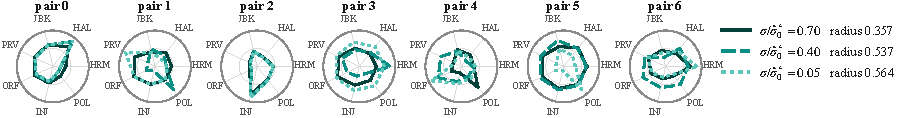
\includegraphics[width=\textwidth]{fig_positions.pdf}
\caption{Where each pair ends up, at three reaches. One radar per pair, seven axes each, coordinates
normalised to $[0,1]$. At $\sigma/\sigma_0^*=0.70$ the polygons are small and similar to one another;
at 0.40 and 0.05 they are larger and distinct, and those two are hard to tell apart.}
\label{fig:positions}
\end{figure}

Below about $\sigma/\sigma_0^*=0.55$ the margin is a plateau between $-0.061$ and $-0.092$ with no
trend, and the apparent optimum at 0.20 does not survive replication (Section~\ref{sec:limits}). The
third panel of Figure~\ref{fig:sigmanll} says what the specialists are actually doing. Own-axis NLL
is flat at 1.79 to 1.82 across the entire sweep while other-axis NLL rises monotonically from 2.007
to 2.39. Shorter reach does not make a pair better on the axis it owns. It makes it worse everywhere
else, and that is what separates the pairs and what the router exploits.

\section{Where the agents start}
\label{sec:init}
Every arm above begins from positions produced by a gradient-ascent solve of the game against the
resource density $B$. We have since established that the $B$ those solves saw was close to uniform
over the lattice: the kernel estimate normalised each grid cell by its own nearest-prompt kernel
value, which flattens the density it was meant to measure. The shipped initialisation is therefore
best described not as an approximate equilibrium but as an \emph{uninformative start} --- a
near-uniform prior over the grid rather than a solution to the game on the prompt cloud. Measured on
the lattice, its coordinate variance is 0.159 with anisotropy 1.29, against 0.084 and 3.10 for the
actual prompt cloud.

This is correctable offline. Solving the same game against the empirical prompt measure gives the
equilibrium the theory actually prescribes, and because the equilibrium depends on the trait cloud
rather than on how it is partitioned, the resulting positions can be dropped into the pipeline with
one factor moved and everything else --- split, $\sigma$, round budget, routing rule, generalist ---
held fixed. Table~\ref{tab:init} reports that substitution across pair count.

\begin{table}[t]
\centering
\caption{Naive start against the game equilibrium at $\sigma/\sigma_0^*=0.50$, by number of pairs
$K$. Margins are router $-$ pooled, more negative better; every cell is scored on the same test
partition against the same generalist, so the difference column is a paired within-prompt contrast.}
\label{tab:init}
\small
\begin{tabular}{lcccccccc}
\toprule
$K$ & 2 & 3 & 4 & 5 & 6 & 7 & 8 & 9 \\
\midrule
Naive start   & $+0.0011$ & $-0.0173$ & $-0.0272$ & $-0.0754$ & $-0.0818$ & $-0.0693$ & $-0.0762$ & $-0.0781$ \\
Equilibrium   & $-0.0247$ & $-0.0303$ & $-0.0635$ & $-0.0700$ & $-0.0830$ & $-0.0726$ & $-0.0734$ & $-0.0816$ \\
\midrule
Difference    & $-0.0258$ & $-0.0130$ & $-0.0363$ & $+0.0054$ & $-0.0012$ & $-0.0033$ & $+0.0028$ & $-0.0035$ \\
\bottomrule
\end{tabular}
\end{table}

The effect is a step, not a trend. At $K \le 4$ the equilibrium start is worth 0.013 to 0.036 NLL; at
$K \ge 5$ the five arms scatter around zero with mean $-0.000$ and SD 0.0039. Those five nulls supply
a measured noise floor rather than an assumed one, against which the three effects below the step are
6.6, 3.3 and 9.2 standard deviations. Two consequences follow. First, at $K=2$ the starting positions
decide whether routing helps at all: the naive start loses to the generalist ($+0.0011$) and the
equilibrium beats it ($-0.0247$). Second, the capacity threshold itself moves. The naive ablation
jumps between $K=4$ and $K=5$; started at the equilibrium, $K=4$ already reaches $-0.0635$, most of
what the naive start needed five pairs to achieve. Part of ``you need at least five pairs'' was a
property of the initialisation rather than of the method.

\paragraph{The equilibrium is an attractor, not just a better guess.} The position update never
consults an adapter, so its behaviour is checkable directly, and the check is the strongest
confirmation of the game model we have. Table~\ref{tab:drift} measures, at every reach, how far the
pairs travel and where they end up relative to the equilibrium. Arms started \emph{at} the
equilibrium barely move: a mean of 0.0153 over twelve rounds, within a narrow 0.0108--0.0183 across
the whole sweep, with straightness 0.12 --- below the 0.30 expected of a random walk, so consecutive
steps are anti-correlated and the pairs are jittering in place on batch noise rather than going
anywhere. That is the theory's own prediction, since $\hat{x}_i = x_i$ is algebraically
$\nabla_{x_i} u_i = 0$.

The naively started arms are the more informative half. They begin a mean of 0.330 away from the
equilibrium in matched $L_2$, travel 0.291 during training, and finish 0.090 away --- closing
\textbf{73\% of the distance to an equilibrium they were never given}, and moving closer in
\textbf{ten arms out of ten}. The competition finds the game's solution on its own, from an
uninformative start, using only gradient information from the prompts it wins. Training moves the
pairs about nineteen times as far when they start away from the equilibrium as when they start on it,
which is what an attractor looks like.

\begin{table}[t]
\centering
\caption{Position drift over twelve rounds, by reach, seed 0. Distances are mean matched $L_2$ in the
seven-dimensional unit box. ``To equilibrium'' is measured against the solve on the empirical prompt
measure; pair index is not an identity across two separate solves, so pairs are matched before
differencing.}
\label{tab:drift}
\small
\setlength{\tabcolsep}{4pt}
\begin{tabular}{lcccccccccc|c}
\toprule
$\sigma/\sigma_0^*$ & 0.05 & 0.10 & 0.20 & 0.30 & 0.40 & 0.45 & 0.50 & 0.55 & 0.60 & 0.70 & mean \\
\midrule
\multicolumn{12}{l}{\emph{Naive start}} \\
distance travelled      & 0.395 & 0.316 & 0.277 & 0.218 & 0.330 & 0.298 & 0.253 & 0.292 & 0.262 & 0.270 & 0.291 \\
start to equilibrium    & 0.427 & 0.347 & 0.321 & 0.242 & 0.340 & 0.367 & 0.275 & 0.335 & 0.298 & 0.351 & 0.330 \\
end to equilibrium      & 0.049 & 0.161 & 0.193 & 0.036 & 0.034 & 0.127 & 0.038 & 0.066 & 0.070 & 0.123 & 0.090 \\
gap closed              & 89\% & 54\% & 40\% & 85\% & 90\% & 66\% & 86\% & 80\% & 76\% & 65\% & 73\% \\
\midrule
\multicolumn{12}{l}{\emph{Equilibrium start}} \\
distance travelled      & 0.018 & 0.018 & 0.017 & 0.016 & 0.016 & 0.015 & 0.014 & 0.014 & 0.013 & 0.011 & 0.015 \\
\bottomrule
\end{tabular}
\end{table}

Two qualifications. The residual 0.090 is not zero, so twelve rounds do not fully reach the
equilibrium, and it varies by reach in a way we cannot yet account for --- from 0.034 at
$\sigma/\sigma_0^*=0.40$ to 0.193 at $0.20$. And convergence toward the equilibrium is not the same
as convergence toward better performance: at $K \ge 5$ pairs the two initialisations reach
statistically indistinguishable margins despite starting a third of the box apart, which is the
geometric counterpart of the step in Table~\ref{tab:init}. Where the agents end up is predicted by
the game; whether that prediction is worth anything depends on whether the naive dynamics had enough
capacity to get there unaided, and above the threshold they do.

\paragraph{The equilibrium does not raise the mean across reach.} Repeating the substitution across
all ten $\sigma$ settings gives a mean paired difference of $-0.0007$ (median $-0.0027$), with the
equilibrium ahead at eight of ten. What it changes is the \emph{shape} of the reach response rather
than its level. Measuring mean $|$second difference$|$ along the reach axis --- which annihilates
trends and so isolates zigzag --- the naive sweep scores 0.0164 and the equilibrium sweep 0.0021, a
factor of 7.8; on the mixture metric the ratio is 4.5, and there the equilibrium curve rises
monotonically with reach in seven of eight steps against the naive curve's four. A standard deviation
does not show this on the mixture metric, because both curves carry a real upward trend in $\sigma$
that SD charges as scatter.

We are deliberately cautious about the cause. The two sweeps are not constructed alike: each naive
arm re-solves from a fresh random start at its own $\sigma$, so adjacent reaches begin 0.302 apart in
mean matched $L_2$ and occupy six distinct axis-sets across the ten arms, whereas the equilibrium
arms begin 0.014 apart and share one axis-set at eight of ten. The smoothness may therefore be a
property of how the family was built rather than of equilibrium as such, and the obvious bridge fails
--- within the naive family, larger position steps do not predict larger changes in margin
(Spearman $\rho = -0.40$, $n=9$). The control that separates the two accounts is to repeat the naive
sweep with positions held fixed across $\sigma$, and it has not been run.

\section{Which ensemble number to report}
\label{sec:mixture}
Everything above reports the \emph{expected} NLL, $\sum_p G_p \cdot \mathrm{NLL}_p$, which is the loss
of committing to one expert drawn according to the router's weights. That is the right quantity for a
system that must pick, and it is what a top-1 or top-$k$ MoE actually pays. It is not, however, what
``ensemble'' normally means. Combining the experts' predictions gives the sequence-level mixture
\begin{equation}
\mathrm{mix}_i \;=\; -\frac{1}{n_i}\,\log \sum_p w_p \exp\!\big(-n_i\,\mathrm{NLL}_{p i}\big),
\label{eq:mixture}
\end{equation}
for prompt $i$ of $n_i$ tokens, reduced the same way as pooled and expected so the numbers stay
comparable. Jensen's inequality orders the three: oracle $\le$ mixture $\le$ expected, always. We
verified this holds on every scored run, which is a theorem and therefore a usable bug check.

Reporting the mixture raises the headline margin on the dense arm from $-0.0693$ to $-0.1095$
--- that is, from 3.4\% to 5.4\% of the pooled NLL --- and changes one qualitative conclusion, the
hard-routing sign discussed in Section~\ref{sec:routing}. We report both throughout rather than
choosing, because they answer different questions, and we flag the weakness of the mixture
explicitly. Equation~\ref{eq:mixture} is a post-hoc reweighting of \emph{completed} sequences. It is
not token-level mixing at generation time, which is what a deployed ensemble would need and which
requires per-token distributions from every expert. The weights also enter only as $(-\log w_p)/n_i$,
so their influence shrinks as sequences lengthen; at the measured mean of 68.2 test tokens they still
matter, as the uniform column shows, but a corpus of long generations would compress the gap between
learned and uniform weighting.

\section{Model scale}
\label{sec:scale}
We repeat the $\sigma/\sigma_0^*=0.50$ arm on five base models, each with its own data-matched
generalist. Absolute NLL is not comparable across tokenizers, so we report the relative margin.

\begin{table}[t]
\centering
\caption{Base model sweep at $\sigma/\sigma_0^*=0.50$. Each row has its own generalist. Gemma-3-1B is
excluded from the trend: its generalist had not converged at twelve rounds, which inflates the
margin.}
\label{tab:scale}
\small
\begin{tabular}{lcccccc}
\toprule
Base model & Params & Oracle & Router & Pooled & Gain & Agree. \\
\midrule
Qwen2.5-1.5B & 1.5B & 1.8857 & 1.9459 & 2.0151 & 3.43\% & 0.705 \\
Qwen2.5-3B   & 3B   & 1.8225 & 1.8809 & 1.9439 & 3.24\% & 0.704 \\
Qwen2.5-7B   & 7B   & 1.7587 & 1.8144 & 1.8702 & 2.99\% & 0.696 \\
Llama-3.2-1B & 1.2B & 1.3982 & 1.4446 & 1.4827 & 2.57\% & 0.709 \\
\midrule
\textcolor{gray}{Gemma-3-1B} & \textcolor{gray}{1B} & \textcolor{gray}{1.3980} &
\textcolor{gray}{1.4465} & \textcolor{gray}{1.7501} & \textcolor{gray}{17.35\%$^\dagger$} &
\textcolor{gray}{0.689} \\
\bottomrule
\end{tabular}
\end{table}

The margin falls from 3.43\% to 2.99\% as the base model grows from 1.5B to 7B. Larger models are
better generalists and leave less for specialisation to recover, but the effect is mild over this
range. Llama-3.2-1B at 2.57\% shows the result is not specific to one model family. Router agreement
is between 0.696 and 0.709 for every model, which is a useful check: agreement depends on the trait
space and the positions, and those are properties of the prompts, not of the model being fine-tuned.

One consequence of the design bounds what the method can claim. The competition runs on prompt
coordinates and the resource density, neither of which depends on the model being fine-tuned, so all
five base models converge to the same positions. A larger base model changes what each adapter learns
at a given position, not where the positions are.

\section{Limitations}
\label{sec:limits}
\textbf{Replication is preliminary.} Table~\ref{tab:rep} reports four data splits, each varying both
the run seed and the split seed. Pooled within-$\sigma$ standard deviation of the margin is 0.0069,
under 10\% of the margin itself. Because every $\sigma$ is scored on the same split, paired contrasts
are the right test. The collapse at $\sigma/\sigma_0^*=0.70$ replicates cleanly and strengthens with
the fourth split: $+0.0380$ against the 0.50 arm, $t(3)=14.9$, $p=0.001$, with all four signs
agreeing. The apparent optimum at $0.20$ still does not separate from the 0.50 arm: $-0.0056$,
$t(3)=-0.98$, $p=0.40$, sign disagreeing across splits (Figure~\ref{fig:rep}).

Two revisions to the three-split version of this table. The advantage of $0.45$ over $0.50$, which
looked real at $t(2)=3.1$, does not survive the fourth split: $+0.0044$, $t(3)=1.78$, $p=0.17$. And
the $0.20$ arm needs a more careful statement than ``does not replicate''. It fails to beat the
$0.50$ arm, but it beats its \emph{own split's sweep mean} in all four splits, by $+0.0220$,
$+0.0069$, $+0.0075$ and $+0.0042$. Short reach is therefore reliably good; what does not replicate
is the size of the seed-0 spike, which is roughly three times the other three and is what originally
motivated running replicates at all. We report the region below $0.55$ as a plateau with a mild
short-reach tilt, and we do not claim an argmax: the best arm is a different $\sigma$ in every one of
the four splits ($0.20$, $0.30$, $0.50$, $0.40$).

\textbf{Data-matched is not compute-matched.} With dense allocation the ensemble takes about seven
times the gradient steps of the generalist and holds seven times the adapter parameters. Hard
$k{=}1$ is the compute-matched arm and it loses. A reader who cares about a fixed training budget
should read our result as being about what an ensemble can extract from a fixed \emph{dataset}.

\textbf{The trait space is one encoder's opinion.} All seven axes come from a single embedding model,
and five of them are one-versus-rest benchmark discriminants rather than label discriminants. Those
axes separate benchmarks by origin, which is partly a topic signal. We have not tested whether the
gain survives a different encoder.

\textbf{The resource density is coarse.} With a $3^7$ grid and bandwidth 0.08 the estimate of $B$ is
close to a nearest-cell histogram. It enters the initial position solve and the definition of
$\sigma_0^*$, so a finer grid could shift the reach scale, though not the comparisons within it,
which all use the same $B$.

\textbf{The initialisation used through Section~\ref{sec:scale} is not an equilibrium.} The initial
gradient ascent stops at its 8{,}000-step budget, and the density it was solving against was close to
uniform for the reason given in Section~\ref{sec:init}. We therefore describe it as an uninformative
start. The equilibrium comparison in Section~\ref{sec:init} was run as a separate substitution and
does not retroactively change any arm reported elsewhere in the paper; where the two differ at
$K \ge 5$ they differ by less than the replicate noise.

\textbf{Run-seed variation is unmeasured.} Every replicate varies the run seed and the split seed
together, so no arm has been retrained at a second run seed on the same split. Split-level noise is
bounded by Table~\ref{tab:rep}; retraining noise at fixed $(\sigma, \text{initialisation})$ is not,
and the sub-0.005 differences in Section~\ref{sec:init} at $K \ge 5$ sit inside that unmeasured
quantity. This matters most for the reach-smoothness result, where the natural control --- fixing
positions across $\sigma$ --- would also isolate run-seed effects, since the run seed moves the naive
positions while leaving the equilibrium positions pinned.

\textbf{The mixture is post-hoc, not token-level.} Equation~\ref{eq:mixture} reweights completed
sequences. A deployed ensemble would mix next-token distributions, which needs per-token
probabilities from every expert and is a larger change than a rescoring pass.

\section{Conclusion}
Experts do not have to be given. Placing LoRA adapters in a learned trait space and letting them
compete for prompts produces a partition and a router at once, and the resulting ensemble beats a
generalist trained on the same data by 3.4\%. The design choices that matter are not the ones sparse
MoE would suggest: dense proportional training beats a sparse gate, and weighting the loss by share
is what keeps the router able to tell the experts apart. Competitive reach tunes how sharply the
partition is drawn, and setting it too close to the stability threshold collapses the experts
together. Whether the same mechanism produces useful partitions in spaces built for capability rather
than safety is the obvious next question.

\appendix
\section{Replication across data splits}
\label{app:rep}
Each split varies both the run seed and the data-split seed, so the two sources of variation are
confounded by design: the question is whether a conclusion survives a fresh corpus partition and a
fresh initialisation together, not which of the two moved it. Every split trains its own generalist,
so the pooled level differs between splits and only within-split contrasts are meaningful.

\begin{table}[t]
\centering
\caption{Routing margin (router $-$ pooled) across four replicate splits. Each split has its own
generalist, so the pooled level differs (2.0152, 1.9841, 1.9925, 1.9990) and only within-split
contrasts are meaningful. More negative is better.}
\label{tab:rep}
\small
\begin{tabular}{cccccccc}
\toprule
$\sigma/\sigma_0^*$ & Split 0 & Split 1 & Split 2 & Split 3 & Mean & SD & vs 0.50 \\
\midrule
0.70 & $-0.0371$ & $-0.0453$ & $-0.0408$ & $-0.0397$ & $-0.0407$ & 0.0034 & $+0.0380$ ($t=14.9$) \\
0.50 & $-0.0693$ & $-0.0864$ & $-0.0841$ & $-0.0752$ & $-0.0787$ & 0.0079 & --- \\
0.45 & $-0.0611$ & $-0.0778$ & $-0.0818$ & $-0.0768$ & $-0.0744$ & 0.0091 & $+0.0044$ ($t=1.8$) \\
0.20 & $-0.0917$ & $-0.0846$ & $-0.0823$ & $-0.0789$ & $-0.0844$ & 0.0054 & $-0.0056$ ($t=-1.0$) \\
\bottomrule
\end{tabular}
\end{table}

\begin{figure}[t]
\centering
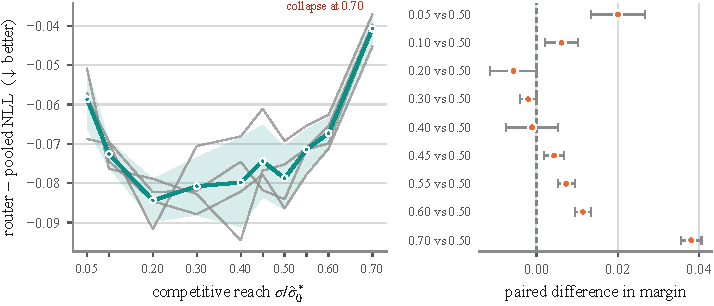
\includegraphics[width=\textwidth]{fig_replication.pdf}
\caption{Left: routing margin against competitive reach. The heavy line is the mean over the four
replicate splits and the band is $\pm1$ SD; the four thin grey lines are the individual splits. Lower
is better, so the curve is a basin: the margin worsens at both ends and is flat between about 0.20
and 0.55. Ticks mark every arm; only the uncrowded ones are labelled. Right: paired differences
against the 0.50 arm, with the standard error over the four splits. The collapse at 0.70 is well
separated from zero and $0.05$ nearly so; $0.20$ is the only reach that improves on $0.50$, and it is
not separable from it.}
\label{fig:rep}
\end{figure}

\section{Base models in detail}
\label{app:scale}
Absolute NLL is not comparable across tokenizers, so Table~\ref{tab:scaledetail} should be read down
a column within a family rather than across families; the margin and the gain are the comparable
quantities. Router agreement is the exception. It depends on the trait space and the positions rather
than on the model being fine-tuned, and it stays between 0.696 and 0.709 for every base model, which
is the check that the routing behaviour itself is model-independent.

\begin{table}[t]
\centering
\caption{Held-out NLL by base model at $\sigma/\sigma_0^*=0.50$, round 11, $n=5{,}671$. Each row has
its own data-matched generalist, so \emph{pooled} differs between rows and only within-row contrasts
are meaningful. \emph{Own} and \emph{other} are the mean NLL on the axis a pair owns under the
optimal one-to-one assignment and on the remaining six, omitted where the per-axis evaluation was not
run. Gain is the margin as a percentage of the pooled NLL. Gemma-3-1B is greyed out: its generalist had not converged at twelve rounds, which inflates both
its pooled NLL and its margin.}
\label{tab:scaledetail}
\footnotesize
\setlength{\tabcolsep}{3pt}
\begin{tabular}{lcccccccccc}
\toprule
Base model & Params & Family & Oracle & Router & Pooled & R$-$P & Gain & Agree. & Own & Other \\
\midrule
Qwen2.5-1.5B & 1.5 & Qwen2.5 & 1.8857 & 1.9459 & 2.0151 & $-0.0692$ & 3.43 & 0.705 & 1.8041 & 2.2282 \\
Qwen2.5-3B & 3.0 & Qwen2.5 & 1.8225 & 1.8809 & 1.9439 & $-0.0630$ & 3.24 & 0.704 & 1.7508 & 2.1693 \\
Qwen2.5-7B & 7.0 & Qwen2.5 & 1.7587 & 1.8144 & 1.8702 & $-0.0558$ & 2.99 & 0.696 & 1.6936 & 2.0895 \\
Llama-3.2-1B & 1.2 & Llama-3.2 & 1.3982 & 1.4446 & 1.4827 & $-0.0381$ & 2.57 & 0.709 & --- & --- \\
\midrule
\textcolor{gray}{Gemma-3-1B} & \textcolor{gray}{1.0} & \textcolor{gray}{Gemma-3} & \textcolor{gray}{1.3980} & \textcolor{gray}{1.4465} & \textcolor{gray}{1.7501} & \textcolor{gray}{$-0.3037$} & \textcolor{gray}{17.35} & \textcolor{gray}{0.689} & \textcolor{gray}{---} & \textcolor{gray}{---} \\
\bottomrule
\end{tabular}
\end{table}

\bibliographystyle{plainnat}
\bibliography{refs}

\end{document}
